% Options for packages loaded elsewhere
\PassOptionsToPackage{unicode}{hyperref}
\PassOptionsToPackage{hyphens}{url}
%
\documentclass[
]{book}
\usepackage{lmodern}
\usepackage{amssymb,amsmath}
\usepackage{ifxetex,ifluatex}
\ifnum 0\ifxetex 1\fi\ifluatex 1\fi=0 % if pdftex
  \usepackage[T1]{fontenc}
  \usepackage[utf8]{inputenc}
  \usepackage{textcomp} % provide euro and other symbols
\else % if luatex or xetex
  \usepackage{unicode-math}
  \defaultfontfeatures{Scale=MatchLowercase}
  \defaultfontfeatures[\rmfamily]{Ligatures=TeX,Scale=1}
\fi
% Use upquote if available, for straight quotes in verbatim environments
\IfFileExists{upquote.sty}{\usepackage{upquote}}{}
\IfFileExists{microtype.sty}{% use microtype if available
  \usepackage[]{microtype}
  \UseMicrotypeSet[protrusion]{basicmath} % disable protrusion for tt fonts
}{}
\makeatletter
\@ifundefined{KOMAClassName}{% if non-KOMA class
  \IfFileExists{parskip.sty}{%
    \usepackage{parskip}
  }{% else
    \setlength{\parindent}{0pt}
    \setlength{\parskip}{6pt plus 2pt minus 1pt}}
}{% if KOMA class
  \KOMAoptions{parskip=half}}
\makeatother
\usepackage{xcolor}
\IfFileExists{xurl.sty}{\usepackage{xurl}}{} % add URL line breaks if available
\IfFileExists{bookmark.sty}{\usepackage{bookmark}}{\usepackage{hyperref}}
\hypersetup{
  pdftitle={Using LANDFIRE Products for FSC compliance},
  pdfauthor={The Nature Conservancy's LANDFIRE team},
  hidelinks,
  pdfcreator={LaTeX via pandoc}}
\urlstyle{same} % disable monospaced font for URLs
\usepackage{longtable,booktabs}
% Correct order of tables after \paragraph or \subparagraph
\usepackage{etoolbox}
\makeatletter
\patchcmd\longtable{\par}{\if@noskipsec\mbox{}\fi\par}{}{}
\makeatother
% Allow footnotes in longtable head/foot
\IfFileExists{footnotehyper.sty}{\usepackage{footnotehyper}}{\usepackage{footnote}}
\makesavenoteenv{longtable}
\usepackage{graphicx,grffile}
\makeatletter
\def\maxwidth{\ifdim\Gin@nat@width>\linewidth\linewidth\else\Gin@nat@width\fi}
\def\maxheight{\ifdim\Gin@nat@height>\textheight\textheight\else\Gin@nat@height\fi}
\makeatother
% Scale images if necessary, so that they will not overflow the page
% margins by default, and it is still possible to overwrite the defaults
% using explicit options in \includegraphics[width, height, ...]{}
\setkeys{Gin}{width=\maxwidth,height=\maxheight,keepaspectratio}
% Set default figure placement to htbp
\makeatletter
\def\fps@figure{htbp}
\makeatother
\setlength{\emergencystretch}{3em} % prevent overfull lines
\providecommand{\tightlist}{%
  \setlength{\itemsep}{0pt}\setlength{\parskip}{0pt}}
\setcounter{secnumdepth}{5}
\usepackage{booktabs}
\usepackage[]{natbib}
\bibliographystyle{plainnat}

\title{Using LANDFIRE Products for FSC compliance}
\author{The Nature Conservancy's LANDFIRE team}
\date{2021-02-15}

\begin{document}
\maketitle

{
\setcounter{tocdepth}{1}
\tableofcontents
}
\hypertarget{landfire-and-the-forest-stewardship-council-us-standards}{%
\chapter{LANDFIRE and the Forest Stewardship Council US Standards}\label{landfire-and-the-forest-stewardship-council-us-standards}}

\hypertarget{softAndData}{%
\chapter{Software and Datasets}\label{softAndData}}

You will need these LANDFIRE products:

\begin{itemize}
\tightlist
\item
  Spatial datasets, clipped to your area(s) of interest

  \begin{itemize}
  \tightlist
  \item
    \href{https://www.landfire.gov/bps.php}{Biophysical Settings}. This dataset will be used to get at ``community habitat'', or where ecosystems could occur based on abiotic factors (e.g., soils, climate).
  \item
    \href{https://www.landfire.gov/sclass.php}{Succession classes} characterizes structural classes on the landscape at the time the dataset represents (e.g., 2016 for LF Version 200).
  \item
    \href{https://www.landfire.gov/evt.php}{Existing Vegetation Type} maps NatureServe's Ecological Systems (see descriptions \href{https://www.landfire.gov/documents/LANDFIRE_Ecological_Systems_Descriptions_CONUS.pdf}{here}).
  \end{itemize}
\item
  Non-spatial products

  \begin{itemize}
  \tightlist
  \item
    \href{http://landfirereview.org/search.php}{Biophysical Settings Descriptions} which has information on natural disturbance regimes and succession class descriptions (also available \href{https://tnc.box.com/s/d3ocvy969s1792m5885filjhktujp86e}{here})
  \item
    \href{https://tnc.box.com/s/d3ocvy969s1792m5885filjhktujp86e}{Reference Condition Table} supplements the BpS descriptions with the ``reference'' percentages for each succession class, for each Biophysical Settings.
  \end{itemize}
\end{itemize}

\hypertarget{gisPrep}{%
\chapter{GIS prep}\label{gisPrep}}

Methods:

\begin{enumerate}
\def\labelenumi{\arabic{enumi}.}
\tightlist
\item
  Once spatial data is clipped to area of interest, perform a ``combine'' in ArcMap (Toolbox \textgreater{} Spatial Analyst \textgreater{} Local \textgreater{} Combine) of the BpS, SCL and EVT datasets. Alternatively, you can combine a raster of the area of interest with those 3 datasets which are stored as larger extents (like shown below).
\end{enumerate}

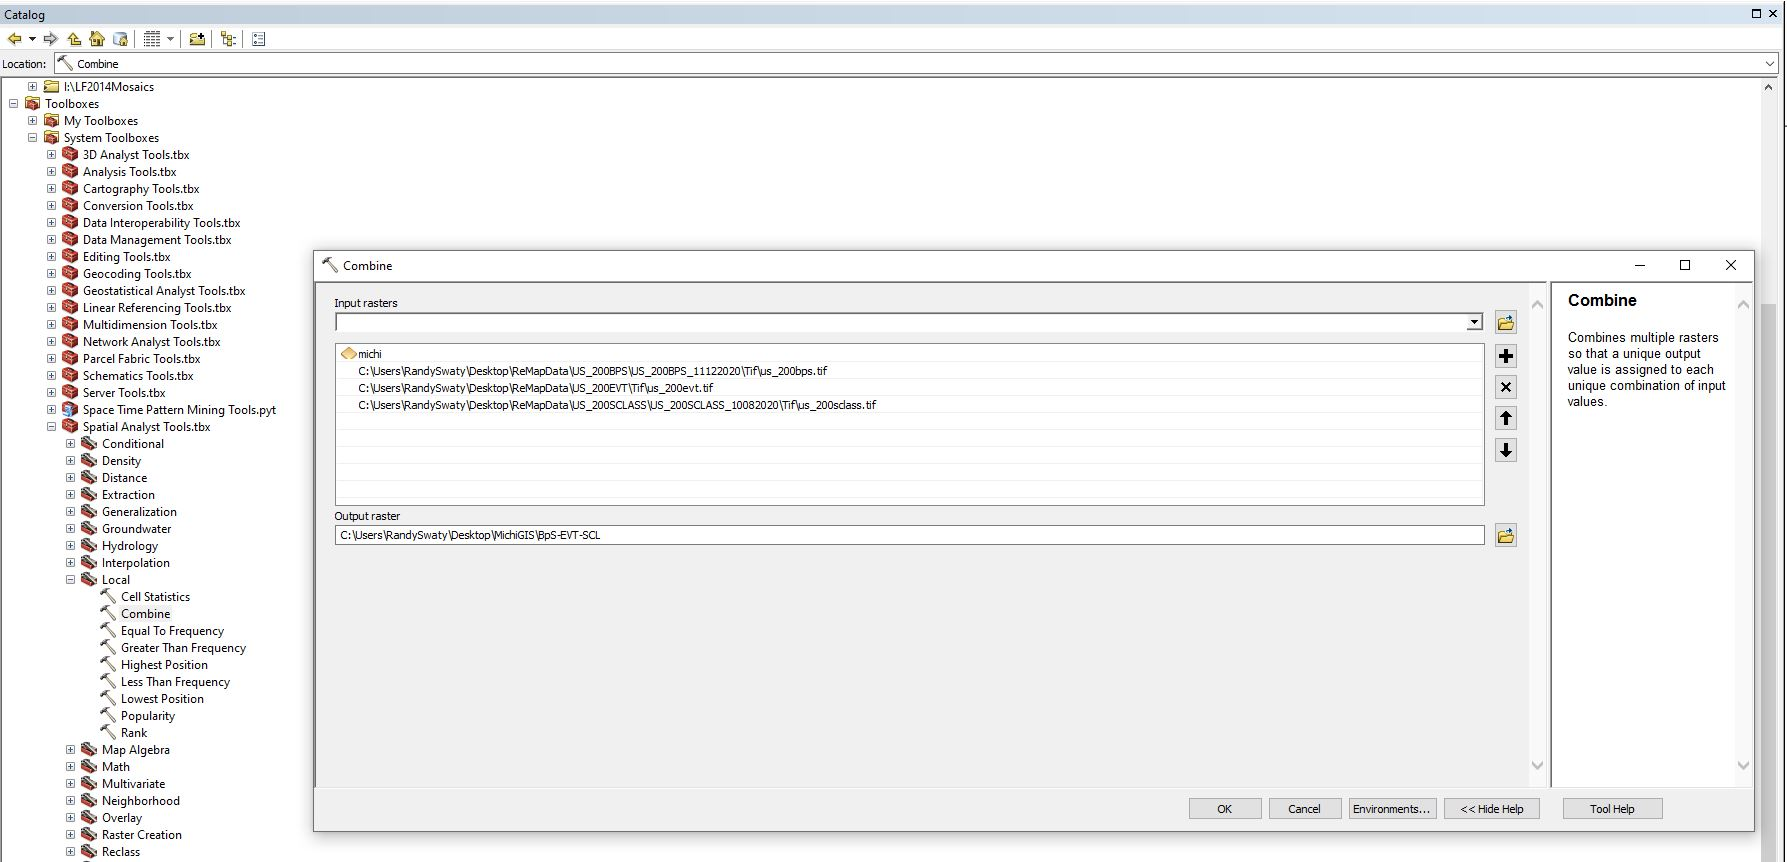
\includegraphics[width=1\linewidth]{combine}

\begin{enumerate}
\def\labelenumi{\arabic{enumi}.}
\setcounter{enumi}{1}
\tightlist
\item
  Join in attributes. There are multiple ways-we recommend using the Join Field tool (Toolbox \textgreater{} data management tools \textgreater{} joins \textgreater{} add join). One reason to do this is to be able to select which fields to join in. A potential resulting table looks like this for a landscape in Michigan (with minimal cleaning/formatting):
\end{enumerate}

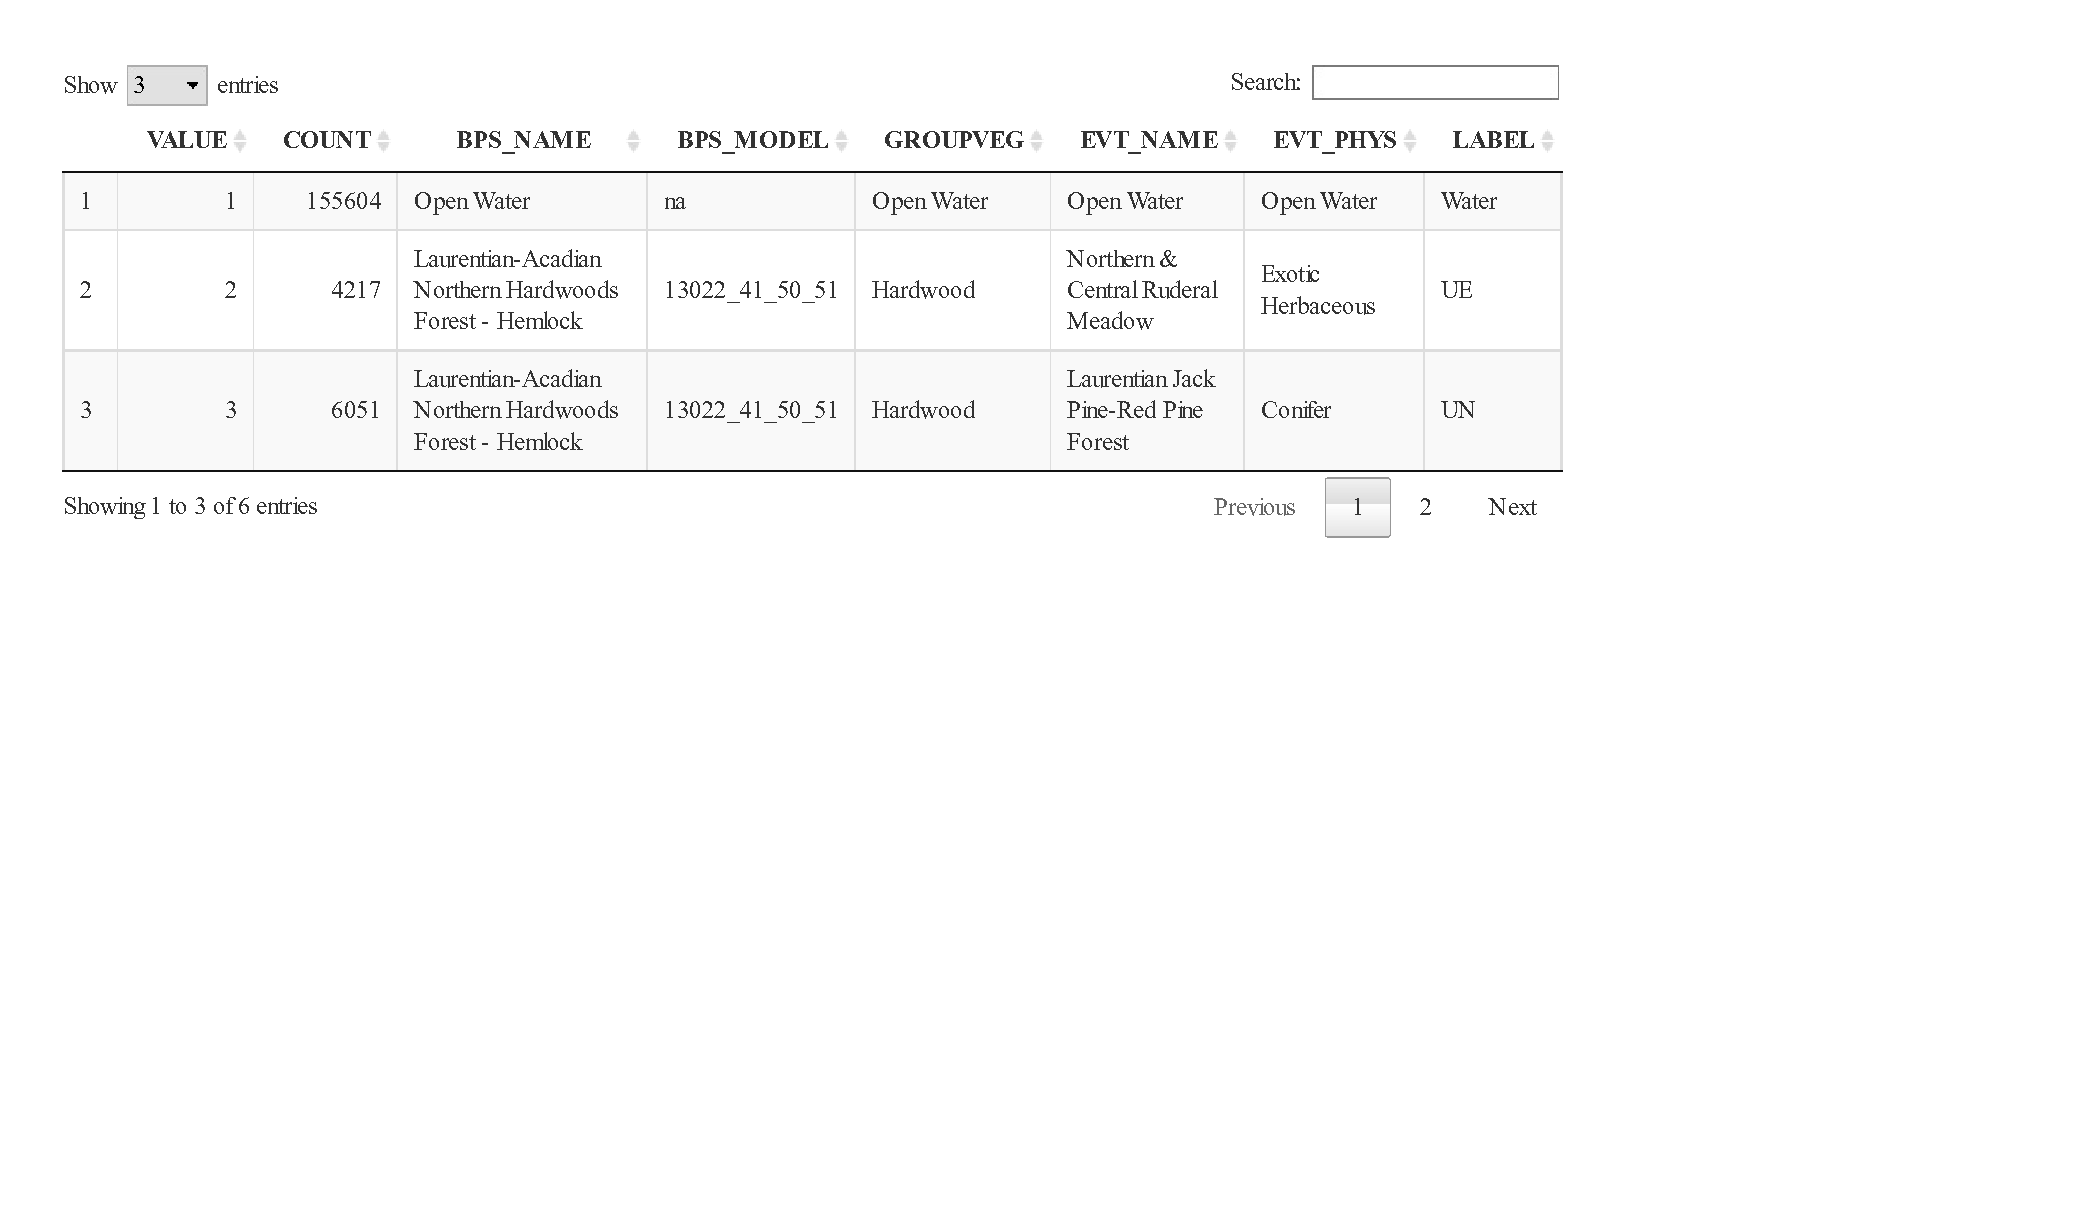
\includegraphics{FSCBook_files/figure-latex/combineDT-1.pdf}

As is this table does not mean too much-we will need to do some cleaning, formatting and calculating.

\begin{enumerate}
\def\labelenumi{\arabic{enumi}.}
\setcounter{enumi}{2}
\tightlist
\item
  Clean data table (combined ``.csv'' file). You will first need to save this file as an ``.xlsx'' file so that you can have multiple worksheets. We recommend keeping the original output as a ``raw'' spreadsheet in Excel, pasting that data into a new sheet and working with that new sheet moving forward.

  \begin{itemize}
  \tightlist
  \item
    It is OK to remove the ``US\_200BPS'', ``US\_200EVT'', and ``US\_200SCLASS'' columns
  \item
    Rename some columns: ``GROUPVEG'' to ``BPSGROUPVEG''; ``EVT\_PHYS'' to ``EVTGROUPVEG''; ``LABEL'' to ``SUCCESSIONCLASS'', or similar as needed for clarity
  \item
    COUNT = number of 30m x 30m pixels for that combination of BpS-EVT-SCLS. Insert a column named ``ACRES'', then calculate acres by multiplying COUNT by ``0.222''. Copy-Paste Values for that new column. Below is an example of what our new data table looks like.
  \end{itemize}
\end{enumerate}

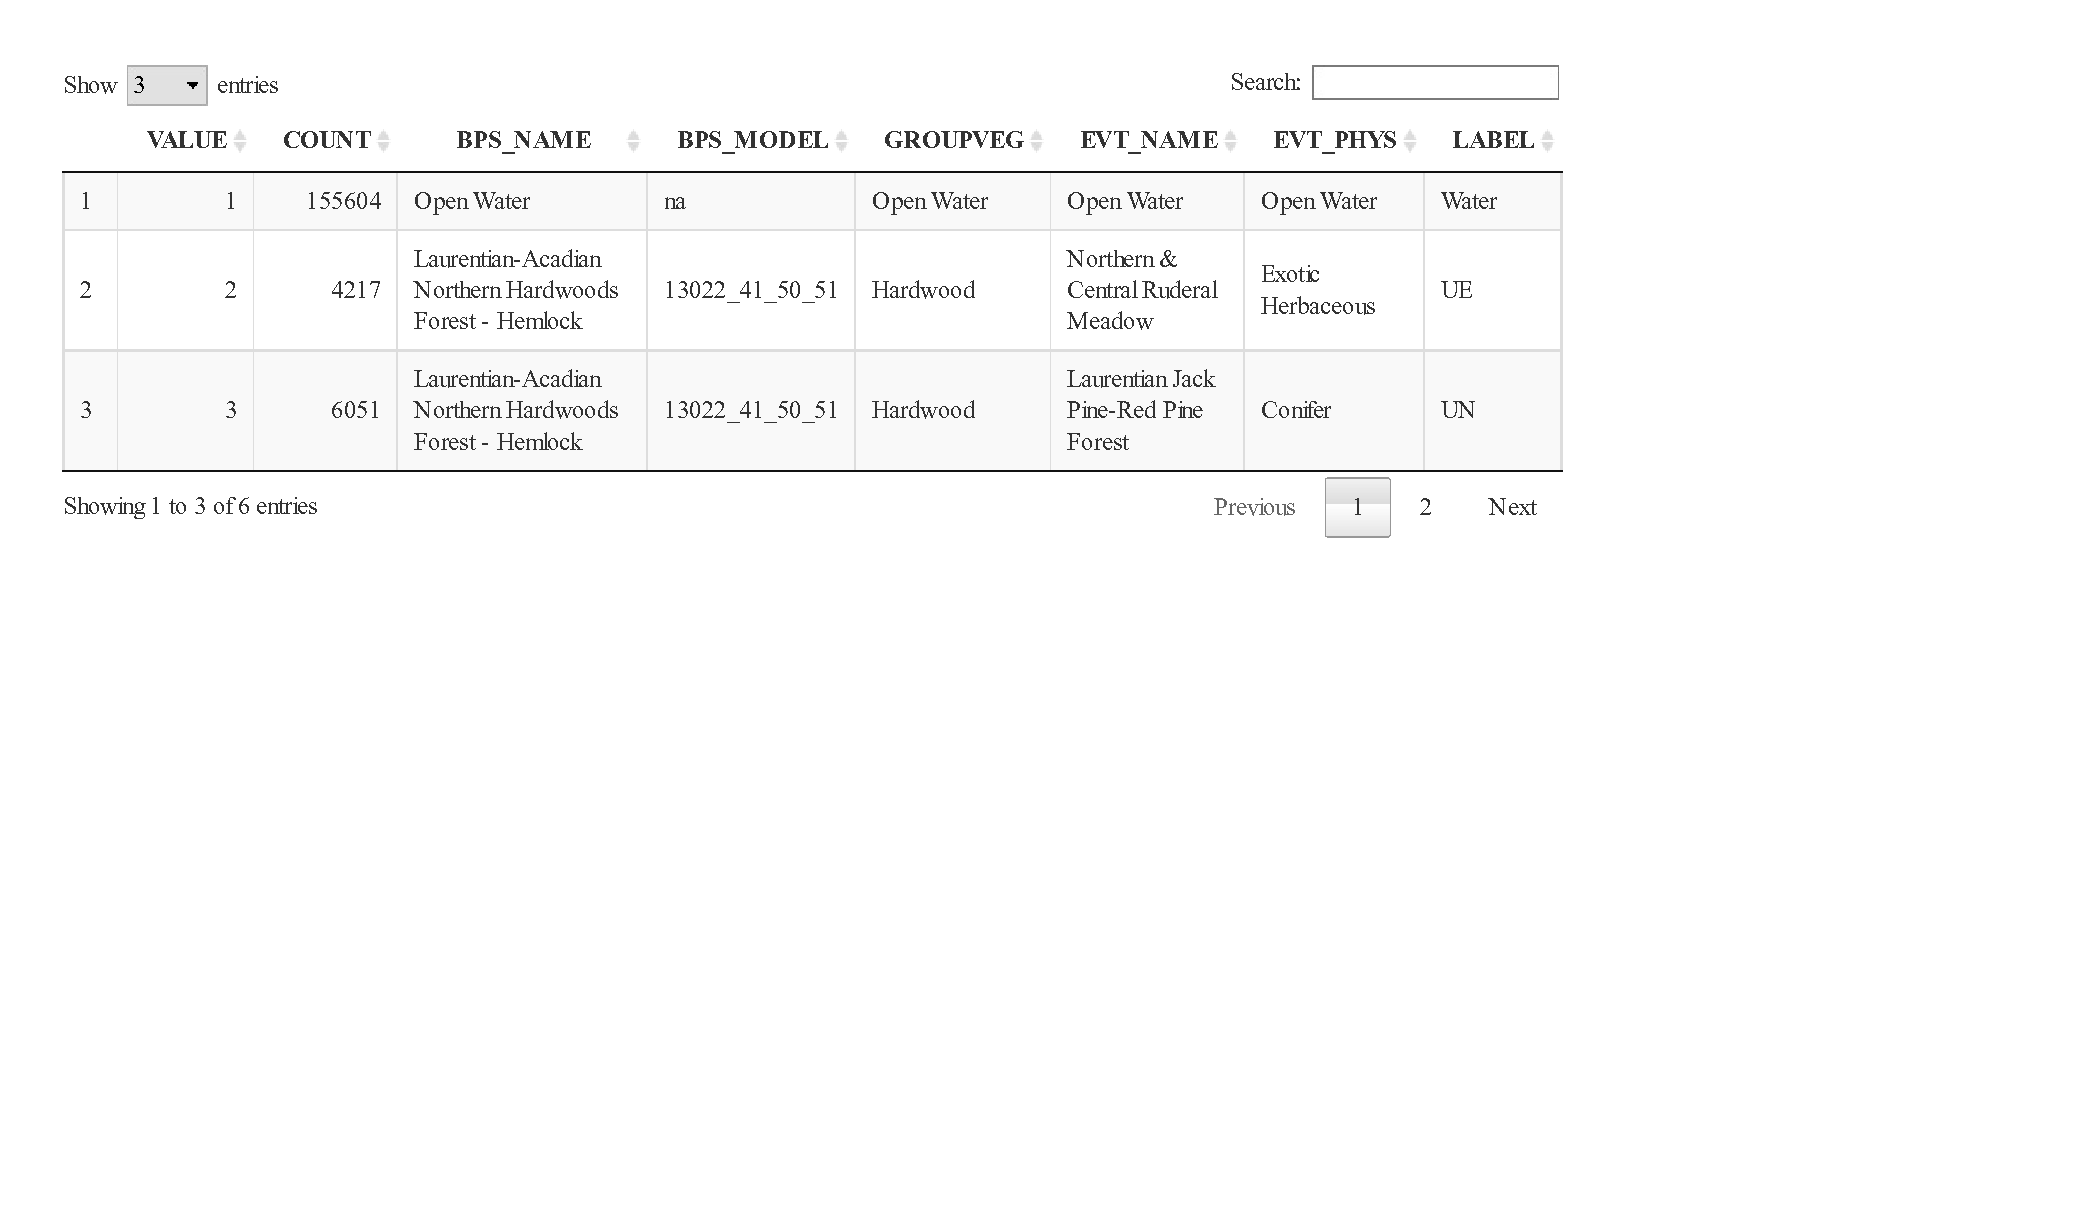
\includegraphics{FSCBook_files/figure-latex/combineCleanDT-1.pdf}

\hypertarget{methods}{%
\chapter{Methods}\label{methods}}

We describe our methods in this chapter.

\hypertarget{applications}{%
\chapter{Applications}\label{applications}}

Some \emph{significant} applications are demonstrated in this chapter.

\hypertarget{example-one}{%
\section{Example one}\label{example-one}}

\hypertarget{example-two}{%
\section{Example two}\label{example-two}}

\hypertarget{final-words}{%
\chapter{Final Words}\label{final-words}}

We have finished a nice book.

\end{document}
